\documentclass[12pt]{article}
\usepackage[utf8]{inputenc}
\usepackage[russian]{babel}
\usepackage{hyperref}
\usepackage{color}
\usepackage{amssymb}
\usepackage{amsmath}
\usepackage{graphicx}
\usepackage{tikz}
\usepackage{titling}
\usepackage{lipsum}
\usepackage{titlesec}
\usepackage{amsthm}

\newtheorem*{theorem}{Теорема}
\newtheorem*{lemma}{Лемма}

\theoremstyle{definition}
\newtheorem*{definition}{Определение}

\titlespacing\section{0pt}{10pt plus 2pt minus 2pt}{0pt plus 2pt minus 2pt}

\setlength{\droptitle}{-10em}   % This is your set screw

\author{Михаил Лепехин и Роман Логинов, группа 694}
\title{Online Convex Optimization (OCO)}

\begin{document}
  \maketitle

\section*{Основные понятия и концепции OCO}

\bigskip
В online выпуклой оптимизации, в отличие от обычной, изученной в курсе, нет фиксированной функции, которую надо минимизировать. Более того, процесс построения оптимального решения делится на несколько итераций. На каждой итерации известны те данные, которые были на предыдущих, а также требуемые для минимизации функции не предыдущих шагах.

Модель напоминает ту, что используется в теории игр. Итерационный процесс позволяет моделировать при помощи OCO процессы, происходящие в действительности.

По шагам это происходит так:

\begin{enumerate}
	\item Игрок (оптимизатор) делает некоторый ход, выдавая вектор $x_t \in \mathcal{K}$
	\item Система (реальный мир) выбирает функцию $f_t \in \mathcal{F}$
	\item На этом шаге вычисляется функция потерь $f_t(x_t)$
\end{enumerate}

Таким образом, на каждой итерации игрок терпит некоторые потери, однако узнаёт новую информацию о функциях. Пусть так будет происходить в течение $T$ итераций.

\bigskip
\textbf{Но в каком случае это вообще имеет смысл?}
\bigskip

Во-первых, хочется, чтобы функции были не совсем произвольными, а \textbf{выпуклыми}, поскольку для их оптимизации существует множество известных алгоритмов.

Во-вторых, на каждом шаге сейчас функция выбирается произвольно и произвольного семейства. Поэтому если оставлять задачу в таком виде, то на каждом шаге система может выбирать неограниченную функцию! И тогда, если на первом шаге функция потерь получилась положительной, то, увеличивая и увеличивая её в дальнейшем, система может не позволить игроку восстановиться от потерь на первой итерации (когда ничего не известно). Таким образом, значение функции потерь должно быть \textbf{ограниченным}.

Наконец, хочется, чтобы \textbf{ограниченным} было и множество $\mathcal{K}$. Конечно, оно может быть не обязательно конечным. Но в случае неограниченного пространства решений система может сопоставлять нулевую потерю для тех значений, которые игрок не выбирает, и огромные в противном случае. А вот, например, шар вполне подходит под такие ограничения (будет использован в дальнейшем)

\bigskip
Теперь формально опишем, чего мы хотим добиться. На каждом шаге мы меняем решение. Но приблизиться мы хотим к оптимальной функции потерь, которая была бы, если бы решение было фиксировано с самого начала. Поэтому для алгоритма $\mathcal{A}$ вводится величина:

$$ regret_T(\mathcal{A}) = \sup\limits_{\{f_1, ..., f_T\} \subseteq \mathcal{F}} \left\{\sum\limits_{t=1}^T f_t(x_t) - \min\limits_{x \in \mathcal{K}} \sum\limits_{t=1}^T f_t(x)\right\} $$

Таким образом, отыскав оптимизирующие $regret$ алгоритмы, мы сможем решать задачи с обновляющейся функцией потерь. Среди примеров обучение на основании советов экспертов, задачи оптимального инвестирования на бирже (portfolio selection) и больше всего приближенная к IT задача фильтрации спама, на примере которой и будут рассмотрены алгоритмы OCO.

\section*{Применение Online Convex Optimisation к задаче фильтрации спама}
$ $

Предположим, что признаки email-сообщений принадлежат множеству $\mathcal{X}$. В качестве признаков будем рассматривать частоты вхождений слов (или групп слов, чтобы размерность мн-ва признаков не получилась слишком большой) в сообщение.

На каждом шаге $t$ функция $a_t : \mathcal{X} \rightarrow [0, 1]$, сопоставляет вектору $x \in \mathcal{X}$ значений признаков некоторое число из отрезка $[0, 1]$. По смыслу это значение является оценкой вероятности (уверенности) того, что сообщение с данными значениями признаков является спамом.

На каждом шаге $t$ соперник выбирает вектор значений признаков $x_t$ и индикатор $y_t$ того, что данное сообщение является спамом.

Для оценки точности метода принятия решений $a_t$ нужно взять некоторую функцию потерь $f_t$. Например, квадратичную функцию потерь:

$$f_t(a_t) := (y_t-a_t(x_t))^2.$$

На каждом шаге функция $a_t(x)$ выбирается из некоторого множества так, чтобы минимизировать $regret$:

$$\sum\limits_{t=1}^T f_t(a_t) - \min\limits_{a \in \mathcal{A}} \sum\limits_{t=1}^T f_t(a) = \sum\limits_{t=1}^T (y_t-a_t(x_t))^2 - \min\limits_{a \in \mathcal{A}} \sum\limits_{t=1}^T (y_t-a(x_t))^2$$


\section*{Применение Online Convex Optimisation к задаче фильтрации спама}
$ $

Предположим, что признаки email-сообщений принадлежат множеству $\mathcal{X}$. В качестве признаков будем рассматривать частоты вхождений слов (или групп слов, чтобы размерность мн-ва признаков не получилась слишком большой) в сообщение.

На каждом шаге $t$ функция $a_t : \mathcal{X} \rightarrow [0, 1]$, сопоставляет вектору $x \in \mathcal{X}$ значений признаков некоторое число из отрезка $[0, 1]$. По смыслу это значение является оценкой вероятности (уверенности) того, что сообщение с данными значениями признаков является спамом.

На каждом шаге $t$ соперник выбирает вектор значений признаков $x_t$ и индикатор $y_t$ того, что данное сообщение является спамом.

Для оценки точности метода принятия решений $a_t$ нужно взять некоторую функцию потерь $f_t$. Например, квадратичную функцию потерь:

$$f_t(a_t) := (y_t-a_t(x_t))^2.$$

На каждом шаге функция $a_t(x)$ выбирается из некоторого множества так, чтобы минимизировать $regret$:

$$\sum\limits_{t=1}^T f_t(a_t) - \min\limits_{a \in \mathcal{A}} \sum\limits_{t=1}^T f_t(a) = \sum\limits_{t=1}^T (y_t-a_t(x_t))^2 - \min\limits_{a \in \mathcal{A}} \sum\limits_{t=1}^T (y_t-a(x_t))^2$$

\section*{Выбор функции $a_t(x)$}
$ $


В машинном обучении для решения задачи классификации спама часто делают следующее. При помощи некоторого алгоритма находят вектор фильтра $a$ из шара $B_R(0)$ относительно некоторой нормы. А после - для определения, является ли сообщение с вектором значений признаков $x$ спамом, рассматривают скалярное произведение $<a, x>$.

Если $<a, x>$ > 0, то сообщение является спамом. Если же знак скалярного произведения отрицательный, то сообщение не является спамом. А если получилось так, что скалярное произведение равно 0, то считается, что тип сообщения не определён.

Будем строить функцию $a_t$ из похожих соображений. Будем также подбирать вектор фильтра $w_t$ из $W := B_R(0)$ и большим значениям скалярного произведения $<w_t, x>$ будет сопоставлять большую вероятность.

В качестве $\mathcal{X}$ возьмём множество векторов $x$ из $\mathbb{R_{+}}^d$, что $\sum\limits_{i=1}^n x_i = 100$ (здесь каждой группе слов сопоставляется процент количества слов из этой группы по отношению ко всем словам в сообщении).

Покажем, что скалярного произведение $<w_t, x>$ ограничено. По неравенству Коши-Буняковского:

$$<w_t, x>^2 \leq ||w_t||_2^2*||x||_2^2 \leq R^2*||x||_2^2 \leq R^2*100^2.$$

Причём, равенство здесь достигается, если сразу выполняются 3 ограничения:

1) $x$ коллинеарен $w_t$ - получим равенство в нер-ве К-Б,

2) $w_t=R$ - получим 2 равенство,

3) $\exists i \in \{1, \dots, d\}: x_i = 100$.

Тогда определим $M := 100R$.

В качестве функции $a_t(x)$ возьмём

 $$a_t(x) = \frac{<x, w_t>+M}{2M}.$$
 
 Тогда функция $f_t$ запишется следующим образом:
 
 $$f_t(x) = \bigg(y_t - \frac{<x, w_t>+M}{2M}\bigg)^2$$
 
\section*{Свойства выбранной функции $a_t(x)$}
$ $

Для нас очень важным свойством будет являться то, что выбранная функция $a_t(x)$ выпукла. Покажем это.

Вычислим её градиент.

$$\frac{\partial f_t}{\partial x}(x) = \frac{2}{2M}(<x, w_t>+M-2My_t)\frac{w_t}{2M} = \frac{<x, w_t>+M-2y_t}{2M^2}w_t$$

Продифференцируем градиент по $x$ и получим гессиан.

$$\frac{2\partial^2 f_t}{\partial x^2}(x) = \frac{1}{2M^2}w_tw_t^T \succeq 0$$

Положительная полуопределённость следует из того, что $\forall x \in \mathcal{X}: x^Tw_tw_t^Tx_t = (w_t^Tx_t)^Tw_t^Tx_t = <w_t^Tx_t, w_t^Tx_t> \geq 0$ - по свойствам скалярного произведения.

По дифференциальному критерию выпуклости 2 порядка функция $f_t(x)$ выпукла. 

\section*{Вычисление regret}
$ $

Для того, чтобы проверять качество работы методов, очень полезно уметь получать значение $regret$.

С учётом выбора функции $a_t(x)$ $regret$ можно записать следующим образом:

$$\sum\limits_{t=1}^T (y_t-a_t(x_t))^2 - \min\limits_{a \in \mathcal{A}} \sum\limits_{t=1}^T (y_t-a(x_t))^2 =$$
$$= \sum\limits_{t=1}^T\bigg(y_t - \frac{<x_t, w_t>+M}{2M}\bigg)^2 - \min\limits_{w \in W}\sum\limits_{t=1}^T\bigg(y_t - \frac{<x_t, w>+M}{2M}\bigg)^2$$

При этом заметим, что $\forall t=1, \dots, T: g_t(w) = \bigg(y_t - \frac{<x_t, w>+M}{2M}\bigg)^2$ является выпуклой по $w$ (доказательство аналогично выпуклости $f_t$ по $x$).
Значит, функция $g(w) = \sum\limits_{t=1}^T\bigg(y_t - \frac{<x_t, w>+M}{2M}\bigg)^2$ является выпуклой как сумма выпуклых функций.

Чтобы получить точное или приближённое значение $regret$ нужно точно или приближённо решить следующую задачу оптимизации:

$$\min g(w)$$
$$s.t. w \in W$$

Эта задача является выпуклой, поскольку:

1) $g(w)$ выпукла в $\mathbb{R}^d$, как было показано выше;

2) множество $W = B_0(R)$ выпукло, поскольку любые 2 точки, лежащие в шаре можно соединить отрезком, каждая точка которого будет также принадлежать этому шару.


Поэтому для получения точного значения $regret$ можно применить теорему Каруша-Куна-Таккера. В силу выпуклости задачи  оптимизации стационарные точки лагранжиана будут точками минимума функции. 

Но нам вполне хватит и приближённого означения $regret$, поэтому для решения вспомогательной задачи оптимизации воспользуемся пакетом $cvxpy$.

\section*{Методы первого порядка}
$ $

В данном разделе мы рассмотрим базовые алгоритмы для Online Convex Optimization, которые достаточно неплохо применимы на практике.

В целом данные методы похожи на соответствующие методы первого порядка для задач обычной выпуклой оптимизации. Но они принципиально отличаются целью применения. Ведь при помощи методов OCO мы стремимся минимизировать не ошибку оптимизации, а \textit{regret}:

$$regret = \sum\limits_{t=1}^T f_t(x_t) - \min\limits_{x \in \mathcal{K}} \sum\limits_{t=1}^T f_t(x)$$

Для сравнения $regret$ с ошибкой оптимизации полезно рассмотреть среднее значение $regret$, т.е. $\frac{regret}{T}$.

Введём обозначение:

$$\overline{x}_T := \frac{1}{T}\sum\limits_{t=1}^T x_t$$

Пусть все функции $f_t$ равны некоторой функции $f : \mathcal{K} \rightarrow \mathbb{R}$, то из неравенства Йенсена получим:

$$f(\overline{x}_T)-f(x^*) = f(\overline{x}_T)- \frac{1}{T} \sum\limits_{t=1}^T f(x^*) \leq \frac{1}{T}\sum\limits_{t=1}^T \big(f(x_t)-   f(x^*)\big	)$$

Таким образом мы показали следующий факт: 

функция $f(x_T)$ сходится к $f(x*)$ не менее быстро, чем среднее значение $regret$.

\section*{Online gradient descent}
$ $

Этот алгоритм, пожалуй, является одним из наиболее интуитивных и простых в Online Convex Optimization. Он базируется на известном нам методе градиентного спуска для offline выпуклой оптимизации.

На каждой итерации этот алгоритм делает шаг от предыдущей точки $x_k$ в направлении градиента предыдущего веса. Но такой шаг может привести к выходу за границу допустимого выпуклого множества $D$. Для того, чтобы этого не произошло, алгоритм проецирует полученную точку обратно на множество $D$, находя ближайшую к ней в $D$.

Псевдокод алгоритма.

Вход: выпуклое множество $\mathcal{K}$, $T$ - размер выборки, $x_1 \in \mathcal{K}$ - начальное приближение, массив со значениями размеров шагов $\alpha_t$.

$\textbf{for}$ $t = 1 \dots T$ $\textbf{do}$

$\textbf{begin}$

$\quad$ Получить $x_t$ и найти значение $f_t(x_t)$

$\quad$ Сделать шаг градиентного спуска.

$\quad y_{t+1} = x_t - \alpha_t \nabla f_t(x_t)$

$\quad$ Спроецировать полученную точку на допустимое выпуклое множество $\mathcal{K}$.

$\quad x_{t+1} = Pr_{\mathcal{K}}(y_{t+1})$

$\textbf{end}$

Выход: значение $x_{T+1}$.

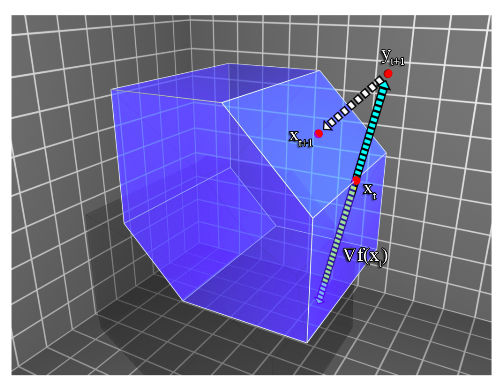
\includegraphics[width=\linewidth]{gradient_descent.png}

\subsubsection*{Нахождение проекции на допустимое множество}

При решении нашей задачи нам нужно будет искать проекцию точки $y_{t+1}$ на $\mathcal{K}$, являющееся шаром радиуса $R$ по евклидовой норме.

Покажем, как это делается.

Нужно решить следующую задачу оптимизации:

$$min ||y-x||_2^2$$
$$s.t.\ x^Tx = R^2$$

Перезапишем квадрат евкидовой нормы в удобном нам виде.

$$min (y-x)^T(y-x)$$
$$s.t.\ x^Tx = R^2$$

1) Если $y_{t+1} \in \mathcal{K}$, то $Pr_{\mathcal{K}}(y) = y$.

2) Решим задачу оптимизации при помощи теоремы ККТ.

	Эта задача выпукла, так как допустимое множество выпукло и оптимизируемая функция является выпуклой как композиция выпуклой и неотрицательной (евклидова норма) и строго возрастающей на неотрицательных значениях ($h(t) = t^2$).
	Значит, найденная стационарная точка лагранжиана даст глобальный условный минимум функции $||y-x||_2^2$.
	
	Итак, запишем лагранжиан.
	
	$$L(x, \mu) = (y-x)^T(y-x) + \mu(x^Tx - R^2)$$	
	
	Для нахождения его стационарных точек, посчитаем градиент.
	
	$$\frac{\partial L}{\partial x}(x, \mu) = 2(1+\mu)x - 2y$$
	
Запишем условие	стационарности.
	
	$$2(1+\mu)x - 2y = 0\ (*)$$ 
	
	Вспомним следующее условие ККТ:
	
	$$\mu(x^Tx-R^2) = 0$$
	
	Это возможно в 2 случаях:
	
	1) $\mu = 0$, откуда из $(*)$ следует $x=y$, что невозможно, так как $y$ не принадлежит допустимому множеству.
	
	2) $x^Tx = R^2$
	
	Значит, $x$ лежит на границе шара $\mathcal{K}$.
	
	Заметим, что все условия ККТ, в том числе, и равенство 0 градиента лагранжиана, выполняются при выборе $x = \frac{y}{||y||_2}$.
	
	Значит, в качестве проекции будем брать именно эту точку.

\subsection{Оценки для online градиентного спуска}
$ $

Будем предполагать градиент каждой из функций $f_t$ ограниченным с константой $G$ (для всего семейства функций).

А также будем рассматривать поведение online градиентого спуска на ограниченных множествах с диаметром $D$ (в нашей задаче используется шар радиуса $R$. Его диаметр равен $2D$).

Несмотря на то, что функция весов на каждом следующем шаге может существенно отличаться от веса на предыдущем шаге, $regret$, получаемый алгоритмом все равно будет сублинейным.

$ $

Это следует из следующей теоремы.

\textbf{Теорема.} Online градиентный спуск с шагом, заданным по правилу $\alpha_t = \frac{D}{G\sqrt{t}}$, для любого $T \geq 1$ гарантирует:

$$regret = \sum\limits_{t=1}^T f_t(x_t) - \min\limits_{x\in \mathcal{K}} \sum\limits_{t=1}^T f_t(x) \leq \frac{3}{2}GD\sqrt{T}$$

$ $

Эта теорема очень важна, поскольку обосновывает применимость метода online градиентного спуска в данной задаче.

Поэтому докажем её.

\textbf{Доказательство.}

Здесь в качестве нормы $||.||$ будем использовать стандартную евклидову норму $||.||_2$.

При доказательстве будем пользоваться следующим вспомогательным утверждением.

\textbf{Утверждение. (Теорема Пифагора)} Пусть $\mathcal{K} \subset \mathbb{R}^d$ - выпуклое множество, $y \in \mathbb{R}^d$ и $x=Pr_{\mathcal{K}}(y)$. Тогда $\forall z \in \mathcal{K}: ||y-z|| \geq ||x-z||$.

Пусть $x^* \in arg \min\limits_{x \in \mathcal{K}} \sum\limits_{t=1}^T f_t(x)$.

Определим $d_t := \nabla f_t(x_t)$.

Из выпуклости функции $f_t(x)$ и дифференциального критерия выпуклости 1 порядка получим:

$$f_t(x_t) - f_t(x^*) \leq d_t^T (x_t-x^*).\ (1)$$

По теореме Пифагора получим:

$$||x_{t+1}-x^*||^2 = ||\Pr_{\mathcal{K}}(x_t - \alpha_td_t) -x^*||^2 \leq ||x_t-\alpha_t d_t-x^*||^2\ (2)$$

Отсюда по неравенству треугольника:

$$||x_{t+1}-x^*||^2 \leq ||x_t-x^*||^2 + \alpha_t^2||d_t||^2 - 2\alpha_td_t^T(x_t-x^*)$$

Учитывая, что $||d_t|| \leq G$ (такое предположение мы делали в самом начале пункта), получим следующую верхнюю оценку.

$$2d_t^T(x_t-x^*) \leq \frac{||x_t-x^*||^2 - ||x_{t+1}-x^*||^2}{\alpha_t} + \alpha_t G^2\ (3)$$ 

Просуммируем неравенства (1) и (3) по $t=1, \dots, T$ и с учётом выбора шага $\alpha_t = \frac{D}{G\sqrt{T}}$, получим:

$$2\bigg(\sum\limits_{t=1}^T f_t(x_t) - f_t(x^*) \bigg) \leq 2\sum\limits_{t=1}^T d_t^T(x_t-x^*) \leq \sum\limits_{t=1}^T 
\bigg(\frac{||x_t-x^*||^2 - ||x_{t+1}-x^*||^2}{\alpha_t} + \alpha_t G^2\bigg)$$
$$= \sum\limits_{t=1}^T 
\frac{||x_t-x^*||^2 - ||x_{t+1}-x^*||^2}{\alpha_t} + G^2 \sum\limits_{t=1}^T \alpha_t \leq $$
$$\leq \sum\limits_{t=1}^T 
||x_t-x^*||^2*\bigg(\frac{1}{\alpha_t}-\frac{1}{\alpha_{t-1}}\bigg) + G^2 \sum\limits_{t=1}^T \alpha_t $$

При последнем неравенстве для удобства положим $\frac{1}{\alpha_0} = 0$

$$\sum\limits_{t=1}^T 
||x_t-x^*||^2*\bigg(\frac{1}{\alpha_t}-\frac{1}{\alpha_{t-1}}\bigg) + G^2 \sum\limits_{t=1}^T \alpha_t \leq $$
$$\leq D^2\sum\limits_{t=1}^T \bigg(\frac{1}{\alpha_t}-\frac{1}{\alpha_{t-1}}\bigg) + G^2 \sum\limits_{t=1}^T \alpha_t = D^2 \frac{1}{\alpha_T} + G^2 \sum\limits_{t=1}^T \alpha_t$$

И, наконец, из выбора шага и того факта, что $\sum\limits_{t=1}^T \frac{1}{\sqrt{t}} \leq 2\sqrt{T}$:

$$D^2 \frac{1}{\alpha_T} + G^2 \sum\limits_{t=1}^T \alpha_t \leq 3DG\sqrt{T}$$
\textbf{Теорема доказана.}

$ $

Кроме того, при выборе шага по данному правилу метод online градиентного спуска является асимптотически оптимальным по значению $regret$.

\textbf{Теорема.} Любой алгоритм для OCO в худшем случае выдаёт $regret = \Omega(DG\sqrt{T})$. Это утверждение верно даже при выборе функции веса из некоторого фиксированного распределения.

$ $

Также стоит отметить, что online gradient descent даёт гораздо более точный результат на сильно выпуклых функциях. Об этом можно судить по следующей теореме.
$ $

\textbf{Теорема.} Для сильно выпуклых функций потерь с константой $\mu$ $online$ градиентный спуск с шагом, выбранным по правилу $\alpha_t = \frac{1}{\mu t}$, гарантирует следующую верхнюю оценку для $regret_T$:

$$regret_{T} \leq \frac{G^2}{2\mu}(1 + log\ T).$$

\section*{Stochastic online gradient descent}
$ $

Одним из случаев online выпуклой оптимизации является стохастическая оптимизация. Как и в стандартной оптимизации, при стохастической оптимизации оптимизатор стремится минимизировать выпуклую функцию $f$, заданную на выпуклом множестве $\mathcal{K}$.

$$\min f(x)$$
$$s.t.\ x \in \mathcal{K}$$

Но в отличие от стандартной оптимизации, алгоритм работает не с градиентом $\nabla_x$ оптимизируемой функции напрямую, а с стохастическим (или зашумлённым) градиентом $\widehat{\nabla}_x$, который является случайной величиной.

При этом, на стохастический градиент накладываются следующие ограничения:
   
1) Несмещённость

   $$\textbf{E}\widehat{\nabla}_x = \nabla f(x)$$
   
2) Ограниченность в среднем

   $$\textbf{E}[\widehat{\nabla}_x^2] \leq G^2$$

*) Для хороших оценок сходимости часто требуют липшициевость стохастического градиента

   $$\widehat{\nabla}_x = O(x)$$

Псевдокод метода online стохастического градиентного спуска.

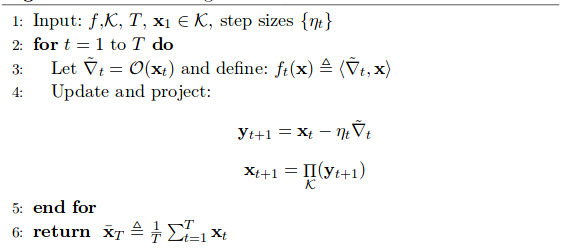
\includegraphics[width=\linewidth]{SGD_algo.png}

Применимость стохастического градиентного спуска в нашей задаче показывает следующая теорема.

\textbf{Теорема.} Стохастический градиентный спуск с размером шага $\alpha_t = \frac{D}{G\sqrt{T}}$ гарантирует:

$$\textbf{E}[f(\overline{x}_T)] \leq \min\limits_{x^* \in \mathcal{K}} f(x^*) + \frac{3GD}{2\sqrt{T}}$$

\section*{Метод Ньютона для OCO}

\subsection*{Экспоненциально вогнутые функции}

\bigskip
Первоначально рассмотрим новый класс функций, не упоминавшийся в курсе - экспоненциально вогнутые (exp-concave) функции. Как мы покажем впоследствии, этот класс более широк, чем сильно выпуклые функции, а значит, когда мы предъявим алгоритм, работающий на этом классе функций, его возможности должны быть шире.

\bigskip
Например, теоремы сходимости для онлайн градиентного спуска показаны только для свойства сильной выпуклости. А в нашем случае такого свойства у функции нет. Также показывается, что аналогичная проблема появляется и при решении задачи protfolio selection.

\bigskip
 
\theoremstyle{definition}
\begin{definition}{Экспоненциально вогнутая с константой $\alpha$ функция}
 - функция $f$, для которой $g = e^{-\alpha f(x)}$ - вогнутая функция.
\end{definition}

Заметим, что в случае сильной выпуклости есть критерий второго порядка: $$\nabla^2 f \succcurlyeq l\mathbf{I}$$

Здесь же суть заключается в том, что гессиан тоже велик, но только в направлении градиента. Покажем критерий второго порядка и в данном случае:

\begin{lemma}
Дважды дифференцируемая функция $f$ экспоненциально вогнута с константой $\alpha \iff \nabla^2 f(x) \succcurlyeq \alpha \nabla f(x) \nabla f(x)^\top$
\end{lemma}

\begin{proof}
Покажем вогнутость через критерий второго порядка. Для этого вычислим гессиан и градиент.

$$ \frac{\partial g}{\partial x_i} = -\frac{\partial f}{\partial x_i} \alpha e^{-\alpha f(x)} $$

$$ \frac{\partial^2 g}{\partial x_i \partial x_j} = \frac{\partial \left(-\frac{\partial f}{\partial x_i} \alpha e^{-\alpha f(x)}\right)}{\partial x_j} = -\alpha \left[ \frac{\partial^2 f}{\partial x_i \partial x_j} e^{-\alpha f(x)} - \alpha \frac{\partial f}{\partial x_i} \frac{\partial f}{\partial x_i} e^{-\alpha f(x)} \right] $$

Сократив на $\alpha e^{-\alpha f(x)}$, получим, что эта матрица является неположительно определённой $\Leftrightarrow$

$$ \nabla^2 f(x) \succcurlyeq \alpha \nabla f(x) \nabla f(x)^\top $$
\end{proof}

Отсюда становится ясно, что сильно выпуклая функция будет и экспоненциально вогнутой. Во-первых, это ясно из интуиции определений. Экспоненциальная вогнутость означает сильную выпуклость лишь в направлении градиента, а значит этот класс функций получается шире. Также это видно и из формулы в лемме. Если $\nabla^2 f \succcurlyeq l\mathbf{I}$, то найдётся $\alpha$, что $\alpha \nabla f \nabla f^\top \preccurlyeq l\mathbf{I}$

Также можно доказать более мощную лемму, которая используется для построения алгоритма:

Обозначим $D$ - диаметр множества $\mathcal{K}$, а $G$ - граница норм градиентов функции $f$

\begin{lemma}
Пусть $f: \mathcal{K} \rightarrow \mathbb{R}$ - экспоненциально вогнутая функция с константой $\alpha$. Тогда для $\gamma < \frac{1}{2} \min\{\frac{1}{4GD}, \alpha\}$ и для всех $x, y \in \mathcal{K}$

$$ f(x) \geqslant f(y) + \nabla f(y)^\top (x - y) + \frac{\gamma}{2} (x - y)^\top \nabla f(y) \nabla f(y)^\top (x - y) $$
\end{lemma}

\subsection{Алгоритм}
$ $

Сам алгоритм будет основан скорее не на методах второго порядка, а всё же на методах первого. Чаще всего в ОСО стандартный алгоритм Ньютона, учитывающий гессиан, не применятся, а используется идея квазиньютоновских методов. На каждой итерации будет использоваться шаг квазиньютоновского алгоритма с матрицей $A_t$, а градиент - это градиент предыдущей функции потерь ($\nabla_t$), вычисленный в сыгранной точке $x_t$.

Для обновления $A_t$ используют следующее правило:

$$ A_t = A_{t - 1} + \nabla_t \nabla_t^\top $$

Тогда можно непосредственно проверить, что:

$$ (A + xx^\top)^{-1} = A^{-1} - \frac{A^{-1}xx^\top A^{-1}}{1 + x^\top A^{-1} x} $$

По индукции ясно, что если взять на изначальном шаге матрицу $A_0 = \varepsilon \mathbf{I}$, то она будет симметричной и неотрицательно определенной на любом шаге как сумма симметричных неотрицательно определенных матриц. Таким образом, обратную матрицу можно отыскать на каждой итерации за квадратичную сложность.

Но шаг метода может вывести нас за пределы $\mathcal{K}$, поэтому применяется аналогичная методу проекций градиента идея. Берётся проекция на множество после каждого шага, но в данном алгоритме не по евклидовой норме, а по норме, порождённой матрицей $A_t$.

Таким образом, на каждом шаге решается следующая задача оптимизации, если после шага получилась точка $y_t$

\begin{align*}
&\min (x - y_t)^\top A_t(x - y_t) \\
s.t.\ & x \in \mathcal{K}
\end{align*}

\textbf{В нашем случае} требуется искать проекцию на шар с центром в нуле. В евклидовой норме это делать легко, а вот по норме матрицы - не так-то просто. Условия ККТ не дают аналитического решения, поэтому будем это делать приближёнными алгоритмами (тот же метод проекций градиента вполне подойдёт)

\begin{theorem}
В обозначениях из леммы выше, описанный выше алгоритм, запущенный с параметрами $\varepsilon = \frac{1}{\gamma^2 D^2}$ и шагом $\frac{1}{\gamma}$ при более чем 4х итерациях гарантирует:

$$ regret_T \leqslant 5(\frac{1}{\alpha} + GD) n \log T $$

Здесь $n$ - размерность матрицы $A$
\end{theorem}
	
\begin{proof}
	Доказательство достаточно громоздкое, его можно найти в указанных в плане источниках.
\end{proof}

Таким образом получили логарифмическую зависимость от числа итераций для экспоненциально-вогнутых функций, что должно быть лучше, чем при использовании онлайн градиентного спуска.

\bigskip
\textbf{Покажем, какая константа для экспоненциальной вогнутости будет в нашем случае:}

Вспомним, как в нашем случае считались гессиан и градиент $f_t(x)$:

$$ \nabla^2 f(x) = \frac{1}{2M^2} w_t w_t^\top $$

$$ \nabla f(x) = \left(\frac{(x, w_t) + M}{2M^2} - \frac{y_t}{2M}\right) w_t $$

Теперь посмотрим на условие первой леммы этого раздела. Рассмотрим 2 случая: $y_t = 0$ и $y_t = 1$. Она говорит, что для подходящего $\alpha$ достаточно:

При $y_t = 0:$

$$ \alpha \left(\frac{(x, w_t) + M}{2M^2}\right)^2 \leqslant \frac{1}{2M^2}$$

$$ \alpha ((x, w_t) + M)^2 \leqslant 2M^2 $$

$$ \alpha \leqslant \frac{2M^2}{((x, w_t) + M)^2} $$

Используя рассуждения предыдущих разделов, по неравенству Коши-Буняковского имеем:

$$ \alpha = \frac{1}{2} \leqslant \frac{2M^2}{((x, w_t) + M)^2} $$

Поэтому можем использовать $\alpha = \frac{1}{2}$

При $y_t = 1:$

$$ \alpha \left(\frac{(x, w_t) + M}{2M^2} - \frac{1}{M}\right)^2 \leqslant \frac{1}{2M^2} $$

$$ \alpha \left(\frac{(x, w)}{2M^2}\right)^2 \leqslant \frac{1}{2M^2} $$

$$ \alpha (x, w)^2 \leqslant 2M^2 $$

$$ \alpha \leqslant \frac{2M^2}{(x, w)^2}$$

Аналогичным образом получаем, что можно использовать $\alpha \leqslant 2$.

Что показывает, что наша функция экспоненциально вогнута с константой $\frac{1}{2}$

\end{document}